\begin{frame}{Salience Estimation and Faithful Generation}

\begin{itemize}

\item Automatic Summarization is an old dream of computer scientists (Luhn, 1958; Edmundson, 1969) 

\vspace{20pt}

\item Traditionally, Summarization researchers and Generation researchers
    (with some meaningful exceptions) have been focused on different goals.

\begin{itemize}

  \item Summarization has been more focused on identifying salient information.
  \item NLG has been more interested in syntactic/semantic representations for
        planning and realizing natural language utterances.

\end{itemize}

\vspace{20pt}

\item \textbf{End-to-End Deep Learning} models of abstractive summarization
    have emerged as a very successful paradigm for performing single document
    summarization (largely independent of these research communities).
        
\end{itemize}
\end{frame}

\begin{frame}[t]{Salience Estimation and Faithful Generation}

\begin{itemize} 
        
\item \textbf{(End-to-End Deep Learning Paradigm)} A Seq2Seq model is trained to map input text to output text directly.
        
        \begin{center}
    
    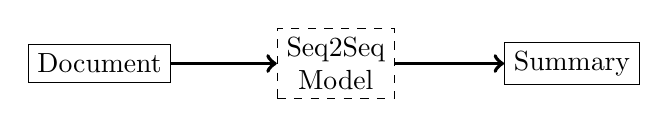
\begin{tikzpicture}
        \node[draw] (doc) at (0,0) {Document}; 
        \node[draw,dashed,align=center] (model) at (3,0) {Seq2Seq \\ Model};
        \node[draw] (sum) at (6,0) {Summary};
        \draw[->,line width=0.5mm] (doc) -- (model);
        \draw[->,line width=0.5mm] (model) -- (sum);
        %\uncover<2->{\node[] (tag) at (4,-0.75) {Whats happening in here?};}
    \end{tikzpicture}
    \end{center}

\only<1-2>{
    \uncover<2->{
    \vspace{10pt}

\item Requires lots of document/summary pairs -- not available for most  domains.

    \vspace{10pt}
\item Difficult to understand why a particular summary was generated.

\begin{itemize}
\item Models may be exploiting dataset specific artifacts or heuristics more
    than they are ``understanding'' the text. (Kry\'sci\'nski et al., 2019)

    \vspace{5pt}

\item Models often hallucinate information/misrepresent the input.
    (Maynez et al., 2020)
    
    \vspace{5pt}

\item Difficult to attribute errors to failures of the language model or
    lack of world knowledge. (Wiseman et al., 2017) 
\end{itemize}

}}

\only<3->{

\item Without explicit justifications for why content was deemed important and
 how that information is to be organized into a summary it seems unlikely that end-to-end abstractive models will be able to address interesting queries like

\begin{itemize}
  \item Summarize a transcript of a doctor's appointment, focusing on evidence
      for a particular diagnosis (that is medically sound).

  \item Summarize last week's Covid-19 news, comparing and contrasting topics
      that were highlighted by news outlets with differing political 
      ideologies.

 \end{itemize}
 \hfill
}
\end{itemize}

\end{frame}

\begin{frame}{Salience Estimation and Faithful Generation}
\begin{itemize}
    
\item In this thesis, we prefer breaking this process up into two steps:

\vspace{10pt}

\begin{center}

\resizebox{0.8\textwidth}{!}{
\begin{tikzpicture}
    \node[draw] (doc) at (0,0) {Document}; 

    \node[draw,align=center,dashed] (ext) at (3,0) {\alert<2>{Extraction} \\ \alert<2>{Model}};
    \node[draw,align=center] (cnt) at (6,0) {Salient \\ Information};
    \node[draw,align=center,dashed] (gen) at (9,0) {\alert<3>{Generation} \\ \alert<3>{Model}};
        \node[draw] (sum) at (12,0) {Summary};
        \draw[->,line width=0.5mm] (doc) -- (ext);
        \draw[->,line width=0.5mm] (ext) -- (cnt);
        \draw[->,line width=0.5mm] (cnt) -- (gen);
        \draw[->,line width=0.5mm] (gen) -- (sum);
        \node at ($(ext)+(-0.35,-1)$) 
            { $ \underbrace{\quad\quad\quad\quad\quad\quad\quad\quad\quad\quad\quad\quad\quad\quad\quad\quad}_{\text{What to say.}}$  };
        \node at ($(gen)+(0.35,-1)$) 
            { $ \underbrace{\quad\quad\quad\quad\quad\quad\quad\quad\quad\quad\quad\quad\quad\quad\quad\quad}_{\text{How to say it.}}$  };
\end{tikzpicture}}
\end{center}

\item<2-> How do learned models of sentence extraction make predictions 
    about sentence salience?
    \begin{itemize}
            \item single document summarization
            \item query focused, stream summarization
            \item neural models and feature based models of salience
    \end{itemize}
    \vspace{10pt}
\item<3->  How to design reliable neural natural language generation (NLG)
    models?
    \begin{itemize}
        \item We study this in an idealized setting where we have a formal
            meaning representation of the content to be realized.
        \item Training methods for faithful and controllable neural NLG models
  \end{itemize}

\end{itemize}

\end{frame}

\begin{frame}{Contributions}
    \begin{itemize}
        \item Salience Estimation with Deep Learning Content Selection
            \begin{itemize}
                \item We show that generic neural architectures are 
                    just as good as task-specific ones.
                \item We show that neural models are strongly influenced by  position heuristics, especially for news.
            \end{itemize}
        \item Salience Estimation with Structured Content Selection Models 
            \begin{itemize}
                \item  On stream summarization task, i.e. where position biases are less useful, we demonstrate the importance of content based features
                \item We propose two approaches to incorporating a salience estimation model into a stream summarization system.
            \end{itemize}
        \item Data Augmentation for Faithful Generation
        \begin{itemize}
            \item We propose noise-injection sampling and self-training scheme that increases semantic correctness of neural NLG model.
        \end{itemize}
        \item Alignment Training for Controllable Generation
        \begin{itemize}
            \item We propose an input transformation to make arbitrary seq2seq models controllable at the level surface order.
        \end{itemize}
    \end{itemize}
\end{frame}

\begin{frame}{Outline}
    \begin{itemize}
        \item[\textbf{Part I.}] \textbf{What to say?}
        \begin{enumerate}
            \item Salience Estimation with Deep Learning Content Selection
                    Models
        \begin{itemize}
            \item single document summarization
            \item neural models
        \end{itemize}
            \item Salience Estimation with Structured Content Selection Models 
        \begin{itemize}
            \item news stream summarization
            \item feature-based models
        \end{itemize}
        \end{enumerate}
        \vspace{10pt}
    \item[\textbf{Part II.}] \textbf{How to say it?}
        \begin{enumerate}
            \item[3.] Data Augmentation for Faithful Generation
            \item[4.] Alignment Training for Controllable Generation
        \end{enumerate}
    \end{itemize}

\end{frame}
